\documentclass[oneside]{ZJUthesis}
% 该文档中首字符为“%”的均为注释行,不会在论文中出现

% 论文默认为单面模式,需单面模式请将第一行换为如下所示:
% \documentclass[twoside]{ZJUthesis}

% 取消目录中链接的颜色,方便打印7778
% 如需颜色,请将“false”改为“true”
\hypersetup{colorlinks=true}

% 这里几行代码使得目录中的“第几章” 和后面的章节名称不致发生重叠
\makeatletter
\renewcommand{\numberline}[1]{%
\settowidth\@tempdimb{#1\hspace{0.5em}}%
\ifdim\@tempdima<\@tempdimb%
  \@tempdima=\@tempdimb%
\fi%
\hb@xt@\@tempdima{\@cftbsnum #1\@cftasnum\hfil}\@cftasnumb}
\makeatother


\begin{document}
%%%%%%%%%%%%%%%%%%%%%%%%%%%%%
%% 正文字体设定
%%%%%%%%%%%%%%%%%%%%%%%%%%%%%
\songti

%%%%%%%%%%%%%%%%%%%%%%%%%%%%%
%% 论文封面部分
%%%%%%%%%%%%%%%%%%%%%%%%%%%%%
% 中文封面内容

% 中图分类号
\classification{TM863}

% 单位代码
\serialnumber{10335}

% 密级,如需密级则将其前“%”去掉
%\SecretLevel{绝密}

% 学号
\PersonalID{11011010}

\title{基于成本的钉耙强度与应用}
% 如果标题一行写不下,就写成两行,在下面的命令里写第二行,不需要两行则注释掉
\titletl{——东方视角分析}

%英文题目
\Etitle{Cost Based Rake Strength}
% 如果一行写不下,同中文题目设定,一行写不下则写两行,不需要就注释掉
\Etitletl{and Application:}
\Etitletll{An Oriental View}

% 作者
\author{猪八戒}
\Eauthor{Bajie Zhu}

\degree{硕士}
\Edegree{Master of Engineering}

% 导师
\supervisor{唐三藏法师}
\Esupervisor{Master Sanzang Tang}

% 合作导师,如果有的话,去掉注释,
% \cpsupervisor{张三丰真人}
% \Ecpsupervisor{Truman Sanfeng Zhang}

% 专业名称
\major{祭坛管理}
\Emajor{Altar Management}

% 研究方向
\researchdm{法器工程}
\Eresearchdm{Ritual Instrument Engineering}

% 所属学院
\institute{大雷音寺管理研究院}
\Einstitute{Management Institute of Great Thunder Monastery}

%论文提交日期
\submitdate{二〇一三年一月十日}
\Esubmitdate{2013-1-10}

% 答辨日期
%\defenddate{2011年11月1日}

% 生成封面
\makeCoverPage

% 生成英文封面
\makeECoverPage

%%%%%%%%%%%%%%%%%%%%%%%%%%%%%%
%% 原创声明与版权协议页
%%%%%%%%%%%%%%%%%%%%%%%%%%%%%%

% 生成原创声明与版权协议页
\makeOSandCPRTpage


%%%%%%%%%%%%%%%%%%%%%%%%%%%%%%
%% 论文部分开始
%%%%%%%%%%%%%%%%%%%%%%%%%%%%%%
\ZJUfrontmatter

%%%%%%%%%%%%%%%%%%%%%%%%%%%%%%
%% 摘要
%%%%%%%%%%%%%%%%%%%%%%%%%%%%%%
\begin{abstract}
人工智能技术的更新正不断影响着人们的生活,近年来愈来愈多的用户采用人机对话的方式来高效地获取优质服务。
跨界服务平台是各类跨界服务集成的支撑系统,将跨越不同行业、组织、价值链等边界的服务进行深度融合和模式创新,
为用户提供多维度、高质量、富价值的跨界服务,成为现代服务业发展的重要创新途径,
相比传统的服务集成,跨界服务融合需开展模式、生态、环境、质量、价值等多维深度融合,
导致内部服务种类繁多、数量庞大,用户在进入系统后,面对如此量级的服务,用户在服务检索时需要花费大量时间,
同时也无法快速查询到与自己意图匹配的服务,因此如何提升用户检索服务时的体验成为问题。

借助人机对话的思想,本文在跨界服务平台中引入服务智能调用引擎。用户进入平台以后,可以输入带有意图的语句,如“查询成都开往杭州的火车票”,
服务智能调用引擎接受语句以后进行包含服务分类、接口分类和参数提取(语义槽填充)三项任务的语义理解,识别并找出系统内部与之匹配的服务,
从句子中提取服务调用必需的参数完成调用返回结果,从而解决了用户检索服务困难的问题。
服务智能调用引擎的核心是语义理解,语义理解模型的性能优劣是衡量调用引擎的智能化程度的重要标准,语义理解的结果也直接影响了服务检索和后续的服务调用。
当前,中文语义理解任务有着诸多困境,如特定下游任务缺乏充分的相关数据集,用户表述意图模糊、随意不规范,一词多义等,因此相关研究受到密切关注,
同时语义理解作为自然语言处理领域的基石性任务,它的研究具有重大科研意义和应用用途。

针对跨界服务领域中文语料匮乏的现状,本文在公开数据集基础上借助搜索引擎和课题组成员人工补充,构建了跨界服务领域的语义理解数据集。
扩充后的数据集包含8个服务类别,每条语料都包含对应的服务类别、接口类别和语义槽标注,共计19145条数据。
同时,本文提出了端到端的服务分类、接口分类和参数提取三项任务交互式联合识别模型,并引入bert作为预训练模型进行微调,
与三项任务独立处理的模型、基于word2vec的模型做了对照实验,验证了模型的可行性和优越性,其中表现最好的bert-co-interactive模型Sentence Acc达到91.47\%。
为将算法应用到实际,依托国家重点研发计划专项《现代服务业共性关键技术研发及应用示范》的子课题《跨界服务集成方法与支撑载体》的原型系统JTangYdrail,
设计了服务智能调用引擎的系统架构,让引擎能与现有平台相结合。

\keywords{跨界服务,文本分类,语义槽填充,意图识别,BERT}
\end{abstract}


%%%%%%%%%%%%%%%%%%%%%%%%%%%%%%
%% 英文摘要
%%%%%%%%%%%%%%%%%%%%%%%%%%%%%%
\begin{englishabstract}
The cross-border service network can break through the traditional organization, business and domain boundaries, 
and has become the main tool to promote cross-enterprise, cross-domain and cross-industry cooperation. 
However, the cross-border service network has a wide variety and huge number of internal services,
users have to spend a lot of cost in service retrieval when facing such a service. 
Therefore, how to improve the user's retrieval service experience becomes a problem. With the help of man-machine dialogue, 
this paper introduces an intelligent service invocation engine into the cross-border service network system. 
The engine can identify? the matching service within the system according to the sentence passed in by the user
and extract the necessary parameters for the service call from the sentence to complete the call and return the result. 
The core of the engine is semantic understanding model. Its performance is an important criterion to measure the degree of engine intelligence, 
and it also directly affects subsequent service calls. At present, Chinese semantic understanding tasks have many challenges, 
such as lack of sufficient data sets for specific downstream tasks, vague user expression intentions, polysemous words, etc. 
At the same time, semantic understanding is the cornerstone of natural language processing, so its research has great significance and application prospects. 

In view of the lack of Chinese corpus in the field of cross-border services, 
this paper builds a semantic understanding data set in the field of cross-border services based on the public data set with the help of search engines and artificial supplements by members of the research team. 
The expanded data set contains 8 service categories, and each corpus contains corresponding service category, 
interface category and semantic slot annotations. At the same time, 
this paper proposes an end-to-end interactive joint recognition model, 
introducing bert as a pre-training model and a knowledge base to enhance the semantics of short text input.
we do control experiments with other models to verify the feasibility and superiority of the model,
Among them, the best-performing bert-co-interactive model's Sentence Acc reached 91.47\%. 
In order to apply the algorithm to practice, 
relying on the prototype system JTangYdrail of the sub-project "Cross-border Service Integration Methods and Support Carriers" of the National Key Research and Development Program "Modern Service Industry Common Key Technology Research and Development and Application Demonstration", 
The system architecture of service intelligent call engine was designed,which allows the engine to be integrated with the existing platform.

\englishkeywords{Natural Language Understanding,Text Classification, Slot Filling, Intent Detection,BERT}
\end{englishabstract}


%%%%%%%%%%%%%%%%%%%%%%%%%%%%%%
%% 目录页
%%%%%%%%%%%%%%%%%%%%%%%%%%%%%%
\ZJUcontents

%%%%%%%%%%%%%%%%%%%%%%%%%%%%%%
%% 插图列表
%%%%%%%%%%%%%%%%%%%%%%%%%%%%%%
\ZJUListofFigures

%%%%%%%%%%%%%%%%%%%%%%%%%%%%%%
%% 表格列表
%%%%%%%%%%%%%%%%%%%%%%%%%%%%%%
\ZJUListofTables


%%%%%%%%%%%%%%%%%%%%%%%%%%%%%%
%% 正文内容部分开始
%%%%%%%%%%%%%%%%%%%%%%%%%%%%%%
\ZJUmainmatter

\chapter{绪论}

\section{课题背景}

依托以互联网为代表的信息技术的高速发展,我国社会当前正处在由传统服务业向现
代服务业全面升级的重要历史进程中。充分利用和结合现代先进的信息技术,提供信息和
知识更加密集、附加值更高的服务是现代服务业的基本要求。互联网作为现代信息服务的
载体,从早期简单的门户网站、搜索引擎,发展到社交网站、即时通信,再到移动搜索、LBS
等移动互联网应用的风靡,在产业规模持续扩大的同时,也不断向各行各业渗透,从早期
的传媒、游戏等行业,到娱乐、零售行业,再到金融、教育和医疗等行业,影响范围还在不
断继续扩大\cite{王晓玲2015我国现代服务业借力}。由此可见,未来服务的基础形态一定是基于互联网的,各行业通过互联网来
提供他们的服务是大势所趋。

跨界服务将跨越不同行业、组织、价值链等边界的服务进行深度融合和模式创新,为用户提供多维度、高质量、富价值的跨界服务,成为现代服务业发
展的重要创新途径。然而,目前针对跨界服务本质规律认知、跨界服务融   
合理论、工程设计方法与运行载体等方面仍然缺少系统研究,缺少充分理
论指导的跨界服务融合实践呈现一定的盲目性,极大影响我国现代服务业
的创新发展。

早期的基于网络的应用服务通常构建于一组相互联系的Web Service 之上。根据W3C
的定义,Web Service 是指用于支持网络内机器之间互操作的软件系统,它通常包含一个机
器可处理的接口描述(一般是WSDL),其它系统按照其接口描述通过SOAP 消息与它进行
交互\cite{verborgh2018web}。Web Service 包含一系列标准化的规范和技术用以支持基于Web 的应用的集成,包
括XML, SOAP, WSDL 和UDDI 等。

Web Service 在早期许多大型企业级软件应用中使用广泛,但由于其相关标准和技术过
于复杂等原因,在如今的新兴互联网应用中已经很少使用了。目前Web API,作为一种更
加灵活和轻量级的解决方案,摒弃了WS 系列的相关复杂标准,得到了广泛的应用\cite{zaveri2017smartapi}。

Web API 如今是Web、物联网、云计算和机器学习应用等的基石\cite{tan2016service}。在Web 应用领域,
随着前后端分离架构的普及,很多Web 应用的界面背后都是由相关的Web API 在直接支
持动态的数据获取和功能访问。在物联网应用中,智能设备和终端也经常会用到诸如广告、
社交网络、消息和支付等Web API\cite{gorla2014checking,viennot2014measurement}。在云计算领域,云服务提供商提供的诸如计算、存
储、消息和数据库等基础服务,都是以Web API 形式供使用者按需调用。在机器学习应用
中,也有许多诸如谷歌翻译这样的Web API,使得开发者无需收集数据、训练模型,也能
直接使用顶尖的图像分类、语音识别和机器翻译等能力。

正是意识到Web API 具有的无限潜能,许多公司选择成立自己的开放平台,开放自家
的部分Web API,一起共建更大的服务生态,实现开放共享、互利共赢。作为最大的Web
API 收录网站,ProgramWeb 网站已经收录了12453 个Web API 和4593 个组合服务。当然
还有许多收费的、企业内部使用的Web API 远远没有收录。Web API 背后所代表的数据和资源,已经促成了所谓API 经济的形成。出现了以京东万象、聚合数据等为代表的各种API
商店。许多供应商仅仅靠提供Web API 就能获得可观的收入,比如SalesForce, AWS。[7]
尽管Web API 目前已经得到了非常广泛的应用,然而在使用Web API 的过程中仍然存
在很多问题。

\begin{figure}[htbp]
  \centering
  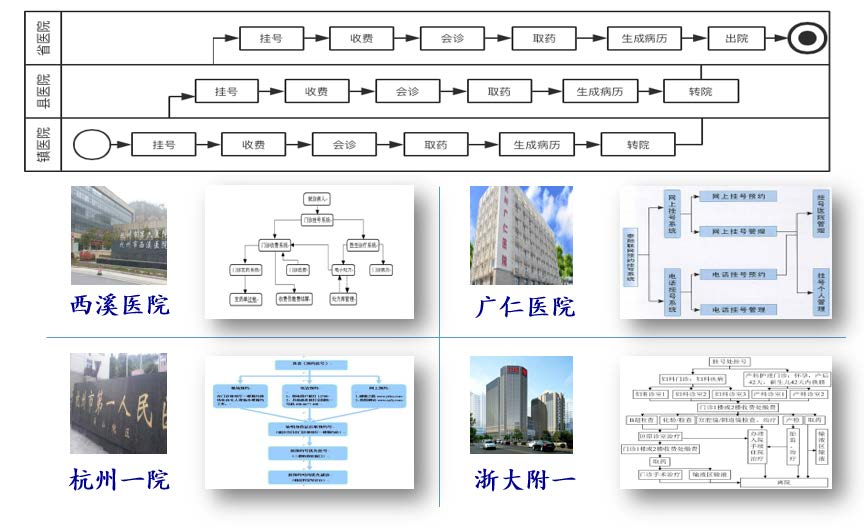
\includegraphics[scale=1]{./images/hospitalRunningModel.jpg}
  \caption{传统医院经营模式下,各家医院标准不一}
  \label{fig:hospitalRunningModel}
\end{figure}

首先,Web API 的描述问题:许多Web API 缺乏有效的描述文档,这给其使用者带来
了很大的障碍。另外,Web API 缺乏统一的描述规范,导致各个公司、组织等都在使用自定
义的、不一致的描述方式,这对于各企业、组织间Web API 的集成和交互式非常不利的,如图\ref{fig:hospitalRunningModel}所展示的,各个地方的医院系统标准不一。再
有就是现在的Web API 描述文档,都是针对人类用户的,缺乏机器可理解性,这对于Web
API 的高效应用,诸如自动组合等方面都是很不利的。

其次,Web API 当前的使用体验问题:用户需要仔细阅读相应的说明文档,然后往往
还需要根据所提供的Web API 的请求和响应等,结合自己的实际需要,进行一层定制或者
包装工作,要正确的使用一个Web API 来获得满足自己需求的结果其实并不容易。

然后,Web API 的选择问题:在很多功能类似的服务中选择一个合适的对很多用户来
说是个挑战。

最后,Web API 的演化问题:服务提供者经常需要升级他们的服务,尽管他们力求做
到向后兼容,但往往还是会或多或少的破坏原来的Web API 接口,服务使用者不得不被迫
修改他们的应用代码以适应新的Web API 的要求,这经常是一项枯燥又繁琐的工作。

本文从服务使用者的角度出发,为解决上述Web API 使用过程中的问题,提出了服务
映射的方法,并开发了相应的系统来支持用户更好的使用服务。

\section{研究意义}
现代服务业是中国经济发展战略中的重要组成部分,也是衡量一个国家经济发展水平
的重要标志。推动现代服务业的发展壮大已成为当前中国经济发展的重要目标和关键动力。
服务计算作为现代服务业发展的重要技术基础,需要结合现代服务业发展的具体场景和具
体问题进行深入的研究和应用。同时,近年来,数字经济已成为全球经济的重要驱动力,“工业+技术”的无限融合不断为市场经济注入新的动力。
在这一发展的浪潮中,企业将大多数业务以Web服务的形式部署在网络中,并为实现复杂业务提供了最基本的功能单元。
最初,这种复杂的业务模型通常是在企业内部实现的,即不同部门根据预定的任务划分提供自己的服务,最终实现复杂而完整的产品。 
但是,随着开发人员要求日益复杂和全球分工明确,单个企业可以提供的服务将不再能满足市场需求。 因此,需要跨企业边界的服务流程来实现业务增值。

本文依托于国家重点研发计划专项《现代服务业共性关键
技术研发及应用示范》的子课题《跨界服务集成方法与支撑载体》,围绕在研究跨界服务集
成和交互过程中发现的Web API 描述文档缺乏、描述方式不一致等导致的集成困难、难以
交互,以及服务使用者使用Web API 过程中遇到的门槛较高、难以上手,需要根据自身需
求进行包装和定制操作,同类服务难以选择,以及Web API 演化导致的应用失败等实际问
题进行了深入的研究和分析,提出了一套以服务映射为基础的解决方案,并
开发了对应的原型系统,不但能够有效解决跨系统的Web API 集成问题,而且提出了以用户为中心的Web API 的使用方式,能够大大简化和改善用户使用Web API 的流程和体验,
还能够避免Web API 演化带来的应用失败的问题,因此本文的研究具有重要的意义。如图\ref{fig:yilianti}
所示,医联体环境下医院经营模式,集成了海量的服务,对用户暴露统一的接口,大大简化了用户的操作。



具体来说,对于一个大型的跨界服务接入平台,当接入的服务数量到达一定阈值时,会出现大量同类型的服务重复接入的情况,比如每一家医院
都有自己的药品查询服务,这一类服务每家医院的名称可能不同,参数可能略有差异,但输入的语义信息都十分接近,可以看作同质服务,
随着接入医院数量的增多,这无疑是一件繁琐且冗余的工作,增加了开发人员的负担而且会有程序漏洞的风险;而且,每个具体的服务参数不同,
对于用户来说,同类型服务下每一个服务就要输入一组参数,而这些参数往往差异不大,简化用户操作无疑势在必行。基于此,
我们提出了服务映射的概念,对于某一类型的服务,在平台内部提出标准服务的概念,标准服务有自己的属性和参数,可在平台内运行,
将该类型同质异构服务自动映射到标准服务,从而快速接入服务,去除繁琐的冗余工作,节约开发成本,
对外暴露统一的标准服务,方便用户,提升用户体验,用户在调用执行标准服务时系统自动映射到实体服务中。

\begin{figure}[htbp]
  \centering
  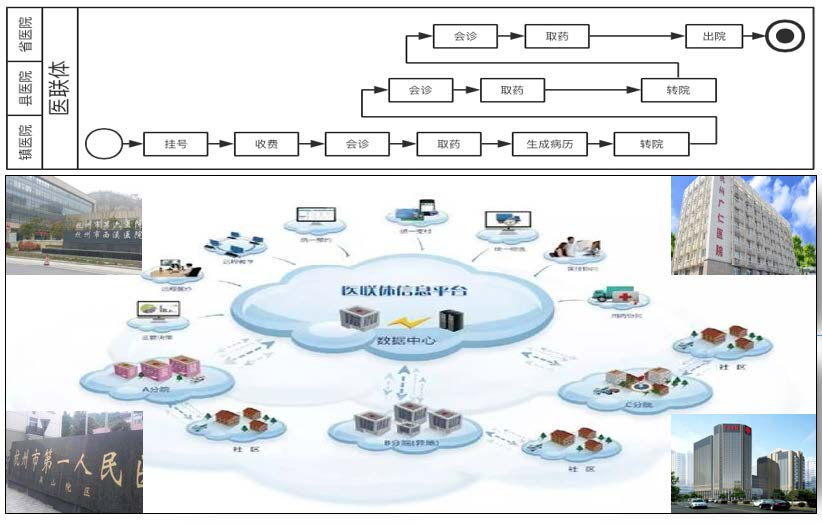
\includegraphics[scale=1]{./images/yilianti.jpg}
  \caption{医联体环境下医院经营模式图}
  \label{fig:yilianti}
\end{figure}

 同时,在当前情况下,当企业想要实施复杂的业务时,如果没有单个Web服务可以满足用户所需的功能,则应该有可能将现有服务组合在一起以满足请求。
 首先需要分析如何将业务划分为几个模块,
 以及每个模块需要什么原子服务。之后,他需要构建服务流程并基于QoS进行服务选择。
 上述两个步骤中的每一个都十分繁琐,并且需要非常丰富的领域专家知识。显而易见,对于这样的一个个流程,当数量达到
 一定阈值时,也会出现上述和标准服务一样的问题:各个服务流程提供商对解决的同一问题呈现出了不同的流程细节,
随着接入流程提供商数量的增多,这无疑是一件繁琐且冗余的工作,增加了开发人员的负担而且会有程序漏洞的风险;而且,每个具体的流程参数、步骤不同,
对于用户来说,同类型流程下每一个服务就要输入一组参数,而这些参数往往差异不大,简化用户操作无疑势在必行。
 本文将同类型(同质)实体流程抽象为标准流程作为统一解决方案,例如医院要发布一站式在线挂号服务的情况,
 该需求大体可以通过“部门信息获取”,“专家信息获取”,
 “注册资源获取”,“注册”和“账单支付”五个功能模块(子服务)对整个业务的服务流程进行建模,可将此作为标准流程构建在跨界
 服务平台。从而实现快速接入流程,去除繁琐的冗余工作,节约开发成本,
 对外暴露统一的标准流程,方便用户,提升用户体验,用户在调用执行标准流程时系统自动映射到实体流程中。


\section{国内外研究现状}

“云大物移智”等新一代信息技术的发展与应用,使得人类的认知扩大、能力增强,
也将重新定义传统边界。“跨界”即突破原有界限,实现界内和界外资源的整合与协作。
跨界服务将跨越不同行业、组织、价值链等边界的服务进行深度融合和模式创新,为用
户提供多维度、高质量、富价值服务,这不仅是技术发展的必然,也是现代服务业发展
的重要创新途径。

相比传统的服务集成,跨界服务融合需开展模式、生态、环境、质量、价值等多维
深度融合,具有极大挑战。目前国内外依然缺少跨界服务本质规模与模式认知、设计与
管理方法、质量管理与价值工程等方面的系统研究,也缺少相关工程方法和支撑载体。
从以下四个方面综述国内外的相关研究:

(1) 服务模式创新是推动现代服务业快速发展的重要因素。近年来,国际上出现
了以Artifact 为中心的商业流程建模方法、基于商业交易过程的商业模式分析框架等,
对服务模式进行了分析和建模;国内浙江大学首次提出了跨界服务概念及其3C 特点。
但总体来看,目前学术界在跨界服务本质规律认知、模式定量分析与评估等方面仍处于
探索阶段。

(2) 跨界服务设计关注如何获取和分析角色多元的用户真实需求,并根据用户需
求进行服务架构、流程和接口等生态设计。IBM 研究院、北京大学、武汉大学等单位的
研究团队在服务需求建模、服务设计和服务互操作性管理等方面具有较好的研究积累,
做出了一系列代表性工作如SOMA-ME、RGPS 需求元建模框架、基于Tropos 的服务建模
方法等,但针对跨界服务融合的设计目前仍缺少完整、系统的支撑方法体系。

(3) 跨界服务融合需要高效、可靠的运行支撑环境,以提供服务网络的运行态支
持。目前这一领域主要有企业服务总线、企业应用集成等相关技术,北京大学、IBM、
佐治亚理工学院等在云端融合资源服务化、服务总线等方面具有较好研究积累,但这些
技术大多针对企业级运行环境,仅实现服务的结构和信息融合,难以应对跨界服务所需
的多维深度融合、动态服务网络优化、开放环境安全管控等挑战。

(4)对服务系统进行精准的能力配置以提供特定的质量与价值,并在运行时准确
感知它们的实际提供水平以做出调控和改进。IBM 研究院、荷兰阿姆斯特丹自由大学、
哈尔滨工业大学等单位的研究团队在服务质量设计与度量、服务价值建模、服务价值感
知等方面具有较好的研究积累,做出了一系列代表性工作,如VASEM、服务价值网等,
但针对跨界服务质量体系和价值工程的研究仍处于初期阶段。

\begin{table}[htb]
  \centering
  \caption{国外从事相关研究的主要机构}
  \label{tab:RelatedResearchAbroad}
    \begin{tabular}{p{4cm}|p{4cm}|p{6cm}}
      \toprule
      % & \multicolumn{1}{m{60mm}}{\heiti\centering 相关研究成果}
      \multicolumn{1}{l|}{\heiti 机构名称} & \multicolumn{1}{l|}{\heiti 相关研究内容} & \multicolumn{1}{l}{\heiti 相关研究成果}\\
      \midrule
      % IBM & 服务科学、服务工程;\\
      IBM & 服务科学、服务工程;& 提出了服务计算研究框架、服务科学、管理与工程体系\\ \hline
       Carnegie Mellon University & 服务测试、组合、推荐等服务计算关键技术 & 提出了服务集成模型、基于语义的服务发现、组合等方法\\ \hline
 University of Sydney & 服务交互模型、服务资源调度、服务质量管理 & 提出了服务质量预测方法、服务组合优化、服务信任度量等方法\\ \hline
 Cambridge Service Alliance,UK & 复杂服务系统、服务使能技术方法&提出了数据驱动复杂业务建模、复杂服务网络管理等方法\\ \hline
 American Service Research & 服务设计、服务质量管理、服务化工程&提出了智能服务设计、服务创新管理等方法\\ \hline
      % \rowcolor[gray]{.9} colortbl & 表格上色。自己看着爽而已,打印出来都是黑白的。 \\
      % threeparttable & 用来给表格添加脚注啥的很方便。 \\
      % array & 忘了用来做什么了,但似乎很重要。 \\
      \bottomrule
    \end{tabular}
\end{table}

\begin{table}[htb]
  \centering
  \caption{国内从事相关研究的主要机构}
  \label{tab:RelatedResearchInChina}
    \begin{tabular}{p{2cm}|p{4cm}|p{8cm}}
      \toprule
      % & \multicolumn{1}{m{60mm}}{\heiti\centering 相关研究成果}
      \multicolumn{1}{l|}{\heiti 机构名称} & \multicolumn{1}{l|}{\heiti 相关研究内容} & \multicolumn{1}{l}{\heiti 相关研究成果}\\
      \midrule
      % IBM & 服务科学、服务工程;\\
      浙江大学 &面向现代服务业的服务计算 &在服务计算相关CCF A 类期刊、会议以及IEEE Trans 上发表论文80余篇,累计GoogleScholar引用超过5000次;获得国家发明专利100 余项。\\ \hline
      武汉大学 &软件服务工程 &主持研制5 项软件服务 相关ISO 国际标准(已 颁布),在IEEE Transactions on Services Computing 和 ICWS 等期刊和会议发 表30 余篇相关论文。\\ \hline
      哈尔滨工业大学 &服务价值工程、 服务质量管理 &提出了价值知觉的服 务工程方法体系,在 IEEE Transactions on Services Computing 和 ICWS,、ICSOC 等相关期 刊和会议上发表30 余 篇相关论文。\\ \hline
      北京邮电大学 &网络服务与智能服务平台 &在IEEE/ACM Transactions 期刊和 CCF A 类会议上发表学 术论文50 余篇,ESI 高 被引文章4 篇,获得国 家发明专利60 余项。\\ \hline
      阿里研究院& 电子商务服务及服务中间件& 探索了电商服务模式,研究数据时代的经济范式,制定了电商服务支撑平台的若干标准,突破了服务组合、服务流程、服务导出等相关的关键技术。\\ \hline
      % \rowcolor[gray]{.9} colortbl & 表格上色。自己看着爽而已,打印出来都是黑白的。 \\
      % threeparttable & 用来给表格添加脚注啥的很方便。 \\
      % array & 忘了用来做什么了,但似乎很重要。 \\
      \bottomrule
    \end{tabular}
\end{table}



关于本文的主要论点:参考服务与参考流程,即服务的映射问题和流程的映射问题,是本文提出的创新性论点
目前国内外暂时没有找到相关研究,但下文会提到,本文把服务和流程的映射问题转化为了nlp领域相对较为成熟
的命名实体识别问题,因此本节接下来简要介绍一下关于命名实体识别的国内外研究状况。

命名实体识别(NER)的任务是识别文本范围内提及的命名实体,并将其分类为预定义的类别,
例如人名,位置,组织等。命名实体是一个单词或短语,
命名实体的示例包括一般域中的组织名称,人员名称和位置名称,生物医学领域中的基因,蛋白质,药物和疾病名称,
NER是将文本中的命名实体定位和分类为预定义实体类别的过程,如图\ref{fig:nerp2}。NER充当各种自然语言应用程序(例如问答系统,文本摘要和机器翻译)的基础。
尽管早期基于统计规则的NER系统成功地产生了不错的识别精度,但是在精心设计规则或功能时,它们通常需要大量的人工。
近年来,通过连续实值矢量表示和通过非线性处理的语义合成的支持,深度学习已被应用于NER系统中,从而产生了最优异的性能。

NER的演变过程,如图\ref{fig:nerp}所示:MUC-6首次使用“命名实体”(NE),
其任务是识别文本中的组织名称,人名和地理位置以及货币,时间和百分比表达式。
自从MUC-6以来,人们对NER的兴趣越来越高,各种测评任务为此主题投入了很多精力。关于问题的定义,
Petasis等限制了命名实体的定义:“ NE是专有名词,充当某物或某人的名称”\cite{petasis2000automatic},
关于NER中应用的技术,主流方法主要有四种:1)基于规则的方法,由于它们依赖手工制定的规则,因此不需要带标注的数据; 
2)无监督学习方法,该方法依靠无监督算法而无需手工标记训练样本; 3)基于特征的监督学习方法,该方法依赖于监督学习算法并经过精心的特征设计; 
4)基于深度学习的方法,该方法以端到端的方式自动从原始输入中发现分类和检测所需的表示形式(特征)。

\begin{figure}[htbp]
  \centering
  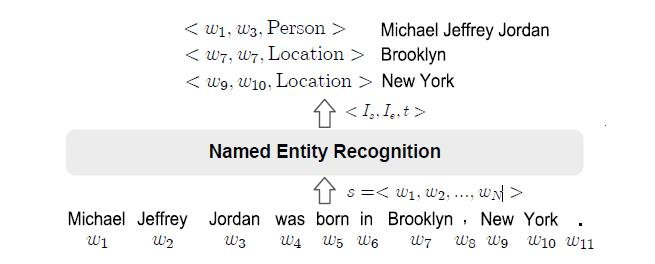
\includegraphics[scale=1]{./images/nerp2.jpg}
  \caption{命名实体识别流程}
  \label{fig:nerp2}
\end{figure}

\begin{figure}[htbp]
  \centering
  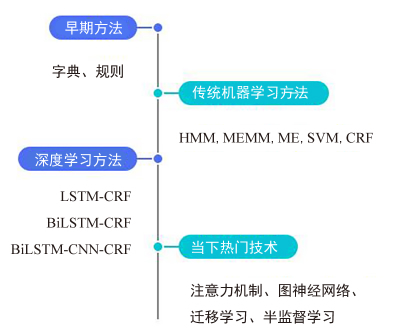
\includegraphics[scale=1]{./images/nerp.jpg}
  \caption{命名实体识别技术研究发展趋势}
  \label{fig:nerp}
\end{figure}

\subsection{基于统计规则的方法}

基于规则的NER系统依赖于人工手动制定的规则,可以基于特定领域的地名词典和句法词法模式设计规则。
Kim等提出使用布里尔规则推理方法进行语音输入,该系统会根据Brill的语音标记器自动生成规则\cite{kim2000rule}。
在生物医学领域,Hanisch等提出了ProMiner,它利用预处理的同义词词典来识别生物医学文本中提及的蛋白质和潜在基因\cite{hanisch2005prominer}。 
Quimbaya等出了一种基于字典的电子健康记录中NER的方法\cite{pomares2016named}。
实验结果表明,该方法在对精度的影响有限的前提下可提高召回率。
其他一些基于规则的知名NER系统包括LaSIE-II,NetOwl,Facile,SAR,FASTUS和LTG系统。
这些系统主要基于手工制定的语义和语法规则来识别实体。当词汇详尽无穷时,基于规则的系统可以很好地工作。
但是,由于特定领域的定制规则和不完整的词典,此类系统中经常会出现高准确率和低召回率的现象,并且这些系统无法很好到迁移到其他域。

\subsection{无监督学习方法}

无监督学习的一种典型方法是聚类,基于聚类的NER系统根据上下文相似性从聚类类簇中提取命名实体,
其核心思想是,可以使用在大型语料库上计算出的词汇资源,词汇模式和统计信息来推断命名实体。 
Collins等观察到,使用未标记的数据将对监督的要求减少到仅需7个简单的“种子”规则\cite{collins1999unsupervised},
然后,作者提出了两种用于命名实体分类的无监督算法。类似地,Etzioni等利用一组谓词名称作为输入,并利用一小组通用提取模式中实现其识别过程\cite{etzioni2005unsupervised}。 
Nadeau等提出了一个非监督系统的地名词典建设和命名实体歧义解决方案,该系统基于简单而高效的启发式方法,结合了实体提取和歧义消除功能\cite{nadeau2006unsupervised}。
另外,Zhang和Elhadad提出了一种从生物医学文本中提取命名实体的无监督方法\cite{zhang2013unsupervised},
他们的模型不是监督,而是求助于术语,语料库统计信息(例如逆文档频率和上下文向量)和浅层语法知识(例如名词短语分块),
在两个主流生物医学数据集上进行的实验证明了其无监督方法的有效性和可推广性。

\subsection{基于特征的监督学习方法}

通过监督学习,NER被转换为多类别分类或序列标记任务。给定带标注的数据样本,特征经过精心设计以能够代表每个训练示例。
然后,利用机器学习算法来学习模型,以从未标注数据中识别出相似的模式。特征工程在有监督的NER系统中至关重要,
特征向量表示是对文本的抽象,其中一个或多个布尔值,数字值代表一个单词。单词级功能(例如大小写,词法和词性标记),
列表查找功能(例如Wikipedia地名词典和DBpedia地名词典),
以及文档和语料库特征(例如,本地语法和多次出现)已广泛用于各种有监督的NER系统。
许多机器学习算法已应用于有监督的NER,包括隐马尔可夫模型(HMM),决策树,最大熵模型,支持向量机(SVM)
和条件随机场(CRF)。 Bikel等提出了第一个基于HMM的NER系统,名为IdentiFinder,用于识别和分类名称,
日期,时间表达式和数字量\cite{bikel1998nymble,bikel1999algorithm}。此外,Szarvas等通过使用C4.5决策树和AdaBoostM1学习算法开发了一种多语言NER系统。
一个主要优点是,它提供了一种可能即可以通过功能的不同子集训练几个独立的决策树分类器,然后通过多数表决方案组合其决策\cite{szarvas2006multilingual}。 
Borthwick等通过应用最大熵理论提出了“最大熵命名实体”(MENE),MENE能够在做出标记决策时利用各种知识资源。
 McNamee和Mayfield使用了1000种与语言相关的功能和258种拼字法和标点功能来训练SVM分类器,每个分类器都会做出二进制决定,即当前令牌是否属于八个类之一\cite{mcnamee2002entity}。
 在预测实体标签时,SVM不考虑相邻词,CRF则考虑了上下文。 
 McCallum和Li提出了NER中CRF的特征归纳方法,在CoNLL03上进行了实验,英文成绩达到了84.04%\cite{mccallum2003early}。 
 Krishnan和Manning提出了一种基于两个耦合CRF分类器的两阶段方法,第二个CRF利用从第一个CRF的输出中得出的潜在表示\cite{krishnan2006effective}。
 此外基于CRF的NER已广泛应用于各个领域的文本,包括生物医学文本和化学文本等。

 \subsection{深度学习方法}

 近年来,基于DL的NER模型逐渐占据主导地位,并取得了最优异的成果,与基于特征的方法相比,深度学习有助于自动发现隐藏的特征。 
 将深度学习技术应用于NER有三个核心优势。首先,NER受益于非线性变换,该变换生成从输入到输出的非线性映射。
 与线性模型(例如对数线性HMM和线性链CRF)相比,基于DL的模型能够通过非线性激活函数从数据中学习复杂的特征。
 其次,深度学习为设计NER特诊节省了大量精力,传统的基于特征的方法需要大量的工程技术和领域专业知识,
 另一方面,基于DL的模型可有效地从原始数据中自动学习有用的表示形式和潜在因素。
 第三,可以通过梯度下降在端到端范式中训练深度神经NER模型,此特性使我们能够设计复杂的NER系统。
 总体的架构如图\ref{fig:nerDL}所示,
 输入的分布式表示形式考虑了单词和字符级别的嵌入,现有的分类法基于字符级编码器,单词级编码器和标签解码器,以及结合了对功能有效的POS标签和地名词典等附加功能,
 上下文编码器将使用CNN,RNN或其他网络捕获上下文相关性,标签解码器为输入序列中的token预测标签。
 例如,在图\ref{fig:nerDL}中,每个token都被预测为带有其类型的命名实体:即带有B-(开头),I-(内部),E-(结束),S-(单个),或O-(外部)的命名实体。
 当然,还有其他标记方案或标记符号,例如BIO。还可以训练标签解码器以检测实体边界,然后将检测到的文本跨度分类为实体类型。

 \begin{figure}[htbp]
  \centering
  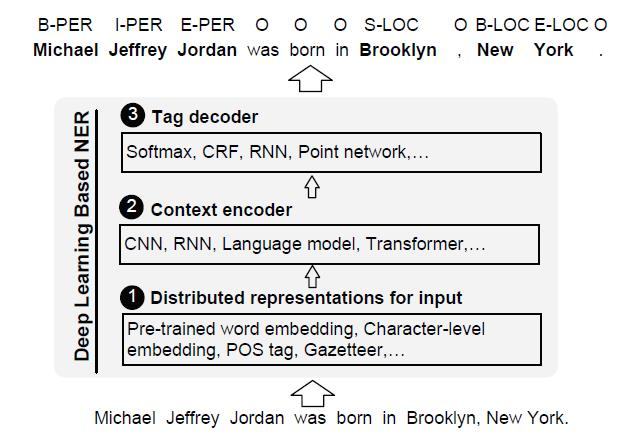
\includegraphics[scale=0.8]{./images/nerDL.jpg}
  \caption{命名实体识别深度学习方法}
  \label{fig:nerDL}
\end{figure}

BiLSTM-CRF是使用深度学习的NER最常见的体系结构。以cloze-style方式预训练双向Transformer模型的方法在CoNLL03上实现了最优异的性能(93.5%)\cite{baevski2019cloze}。 
BERT和dice loss的工作在OntoNotes5.0上达到了最优异的性能(92.07%)\cite{li2019dice}.
NER系统的成功很大程度上取决于其输入的表示形式,集成或微调预训练的语言模型嵌入正成为神经NER的研究热点,
利用这些语言模型嵌入时,可以显着提高性能。
我们从三个角度讨论利弊:输入,编码器和解码器。
首先,关于是否应该使用外部知识或如何将其集成到基于DL的NER模型尚未达成共识,
一些研究表明,外部知识可以提高NER的表现。
但是,缺点也很明显:1)获得外部知识是劳动密集型的(例如地名词典)或计算上昂贵的(例如依赖项); 2)整合外部知识会对端到端学习产生不利影响,并损害基于DL的系统的通用性。
其次,当在大型语料库上对Transformer进行预训练时,Transformer编码器比LSTM更有效。如果未预先训练且训练数据有限,则Transformer将无法完成NER任务\cite{guo2019star,yan2019tener}。
第三,RNN和Pointer Network解码器的主要缺点在于贪婪解码,这意味着当前步骤的输入需要上一步的输出。此机制可能会对速度产生重大影响,并且是并行化的障碍。 
CRF是标签解码器的最常见选择,当采用非语言模型(即非上下文化)嵌入(例如Word2vec和GloVe)时,CRF可以具有强大地捕获标签转换相关性的能力。
但是,当实体类型的数量很大时,CRF在计算上可能会很缓慢。更重要的是,当采用上下文化语言模型嵌入(例如BERT和ELMo )时,与softmax分类相比,CRF并不总是导致更好的性能。
对于最终用户,选择哪种体系结构取决于数据和域任务。如果数据丰富,则可以考虑从头开始使用RNN训练模型,并对上下文语言模型进行微调。
如果数据稀缺,则采用迁移的策略可能是更好的选择。对于新闻专线领域,有许多可用的预训练的现成模型。对于特定领域(例如,医学和社交媒体),
使用特定领域的数据对通用的上下文化语言模型进行微调通常是一种有效的方法。NER适用于不同的语言,主要关注英语和一般领域的NER。
除了英语以外,还有许多其他语言或跨语言环境的研究。
 Zhang 和 Yang 提出了一种针对中文NER的格子结构LSTM模型,该模型对输入字符序列以及与词典匹配的所有潜在单词进行编码\cite{zhang2018chinese}。
 除中文外,许多研究使用其他语言进行,包括蒙古语,捷克语,阿拉伯语,越南语,印度尼西亚语等。
 每种语言都有其自己的特征,可以理解该语言上NER任务的基础,也有许多研究旨在通过将知识从源语言转移到标签很少或没有的目标语言来解决跨语言环境中的NER问题。

迁移学习旨在通过利用从源域中学到的知识来在目标域上执行机器学习任务\cite{pan2009survey},在NLP中,迁移学习也称为领域适应。
对于NER任务,传统方法是通过自举算法。 
Pan等提出了跨域NER的转移联合嵌入(TJE)方法,TJE使用标签嵌入技术将多类别分类转换为低维潜在空间中的回归问题\cite{pan2013transfer}。 
Qu等观察到相关的命名实体类型通常共享词汇和上下文特征\cite{qu2016named},他们的方法使用两层神经网络来学习源命名实体类型和目标命名实体类型之间的相关性,
适用于源域与目标域具有相似(但不相同)的ner问题。 
Peng和Dredze在多任务学习环境中探索了迁移学习\cite{peng2016multi},他们在新闻和社交媒体这两个领域中分别考虑了:分词和NER这两项任务,
在迁移学习的设置中,不同的神经模型通常在源任务和目标任务之间共享模型参数的不同部分。
Yang等首先研究了神经网络的不同层的可迁移性\cite{yang2017transfer},然后,他们针对跨域,跨语言和跨应用程序场景提出了三种不同的参数共享架构。
如果两个任务具有可映射的标签集,则存在一个共享的CRF层,否则,每个任务将学习一个单独的CRF层。
实验结果表明,在资源匮乏的情况下(即更少的可用标签),各数据集的跑分成绩都有了显着改善。 
赵等提出了一种具有领域适应性的多任务模型,其中全连接层适用于不同的数据集,但CRF特征是分别计算的,
赵氏模型的主要优点是,在数据选择过程中会过滤掉分布不同且标注未对齐的实例\cite{zhao2018improve}。



\chapter{假的}

\section{课题背景}

九齿钉耙学名{\kaishu 上宝沁晶耙},是俺的武器。九齿钉耙并非普通的农具,而是由太上老君\footnote{太上老君,三清之第三位。又称“道德天尊”、“混元老君”、“降生天尊”、“太清大帝”等。}用神冰铁亲自锤炼,借五方五帝、六丁六甲之力锻造而成,有诗为证:

7777

% \begin{tabbing}
% \hspace{20mm} \= \hspace{20mm} \= \hspace{80mm} \kill\\
%  \> 字体      \>  \hspace{26mm} 示例 \\
%  \> fangsong \> \fangsong 老君自己动钤锤,荧惑亲身添炭屑。 \\
%  \>          \> \fangsong 五方五帝用心机,六丁六甲费周折。 \\
%  \>          \> \fangsong 造成九齿玉垂牙,铸就双环金坠叶。 \\
%  \> heiti    \> \heiti 身妆六曜排五星,体按四时依八节。 \\
%  \>          \> \heiti 短长上下定乾坤,左右阴阳分日月。 \\
%  \>          \> \heiti 六爻神将按天条,八卦星辰依斗列。 \\
%  \> kaishu    \> \kaishu 名为上宝沁金钯,进与玉皇镇丹阙。 \\
%  \>          \> \kaishu 因我修成大罗仙,为吾养就长生客。 \\
%  \>          \> \kaishu 敕封元帅号天蓬,钦赐钉钯为御节。 \\
%  \> lishu    \> \kaishu 举起烈焰并毫光,落下猛风飘瑞雪。 \\
%  \>          \> \kaishu 天曹神将尽皆惊,地府阎罗心胆怯。 \\
%  \>          \> \kaishu 人间那有这般兵,世上更无此等铁。 \\
%  \> songti   \> \songti 随身变化可心怀,任意翻腾依口诀。 \\
%  \>          \> \songti 相携数载未曾离,伴我几年无日别。 \\
%  \>          \> \songti 日食三餐并不丢,夜眠一宿浑无撇。 \\
%  \> youyan    \> \kaishu 也曾佩去赴蟠桃,也曾带他朝帝阙。 \\
%  \>          \> \kaishu 皆因仗酒却行凶,只为倚强便撒泼。 \\
%  \>          \> \kaishu 上天贬我降凡尘,下世尽我作罪孽。 \\
%  \> default  \> 石洞心邪曾吃人,高庄情喜婚姻结。 \\
%  \>          \> 这钯下海掀翻龙鼍窝,上山抓碎虎狼穴。 \\
%  \>          \> 诸般兵刃且休题,惟有吾当钯最切。 \\
%  \>          \> 相持取胜有何难,赌斗求功不用说。 \\
%  \>          \> 何怕你铜头铁脑一身钢,钯到魂消神气泄!
% \end{tabbing}

\section{各种示例}

没有规定英文字体,将中、英文统一设置为仿宋。

当存在连续多个表格、图片时,\LaTeX 的排版效果不佳,所以这里不时插播些王勃的《腾王阁序》,有空的话也看两眼。

《腾王阁序》第一段:豫章故郡,洪都新府。星分翼轸,地接衡庐。襟三江而带五湖,控蛮荆而引瓯越。物华天宝,龙光射牛斗之墟;人杰地灵,徐孺下陈蕃之榻。雄州雾列,俊采星驰。台隍枕夷夏之交,宾主尽东南之美。都督阎公之雅望,棨戟遥临;宇文新州之懿范,襜帷暂驻。十旬休假,胜友如云;千里逢迎,高朋满座。腾蛟起凤,孟学士之词宗;紫电青霜,王将军之武库。家君作宰,路出名区,童子何知,躬逢胜饯。

《腾王阁序》第二段:时维九月,序属三秋。潦水尽而寒潭清,烟光凝而暮山紫。俨骖騑于上路,访风景于崇阿。临帝子之长洲,得天人之旧馆。层台耸翠,上出重霄;飞阁翔丹,下临无地。鹤汀凫渚,穷岛屿之萦回;桂殿兰宫,即冈峦之体势。披绣闼,俯雕甍:山原旷其盈视,川泽纡其骇瞩。闾阎扑地,钟鸣鼎食之家;舸舰迷津,青雀黄龙之轴。云销雨霁,彩彻区明。落霞与孤鹜齐飞,秋水共长天一色。渔舟唱晚,响穷彭蠡之滨;雁阵惊寒,声断衡阳之浦。

\subsection{图片示例}

附上照片一张,来源 Wikipedia。

\begin{figure}[htbp]
  \centering
  \includegraphics[scale=0.5]{./images/zhubajie.png}
  \caption{玉照,玉做的照片,通常会令人联想到浴照。}
  \label{fig:example}
\end{figure}

我来插两张并排的图像,其实\LaTeX 支持jpg, png, 以及eps格式的图片,图\ref{fig:tangseng}是我的师傅,帅吧!

\begin{figure}[htbp]
\centering
\subfloat[师傅]{
\includegraphics[width=6cm]{./images/tangseng.jpg}
\label{fig:tangseng}
}
\hspace{60pt}
\subfloat[大师兄]{
\includegraphics[width=6cm]{./images/sunwukong.png}
\label{fig:sunwukong}
}
\caption{你挑着担,我写代码...}
\end{figure}

\subsection{表格示例}

\LaTeX 中的表格不是很好搞,看起来很不直观,不过我们一般不会用太高端的表格,更多关于表格的请看\texttt{Helin Gai}的\textsf{\LaTeX Manual}\cite{gaiart}以及
\texttt{Alpha Huang}的\textsf{lnotes}\cite{lnotes}

先看一个简单表格 \ref{tab:simple-table}:

\begin{table}[htb]
  \centering
  \caption{模板中的表格宏包}
  \label{tab:simple-table}
    \begin{tabular}{ll}
      \toprule
      \multicolumn{1}{m{20mm}}{\heiti\centering 宏包} & \multicolumn{1}{m{80mm}}{\heiti\centering 描述} \\
      \midrule
      longtable & 绘制跨页的表格。 \\
      booktabs & 三线表中的那三条线的命令来自这里。\\
      caption2 & 用于设置标题很方便,已经 obsolated,不过 \TeX Live 中还有。\\
      multirow & 跨行的单元格用这个宏包。\\
      dcolumn  & 想让表格小数点对齐吗?用这个宏包吧。\\
      \rowcolor[gray]{.9} colortbl & 表格上色。自己看着爽而已,打印出来都是黑白的。 \\
      threeparttable & 用来给表格添加脚注啥的很方便。 \\
      array & 忘了用来做什么了,但似乎很重要。 \\
      \bottomrule
    \end{tabular}
\end{table}


\subsection{公式示例}

我公式用非常少,所以公式的情况并不了解,这部分示例也完全照搬 。如果有什么问题或要求,可以贴到 88 \TeX 版。

贝叶斯公式如式 (\ref{equ:chap1:bayes}),其中 $p(y|\mathbf{x})$ 为后验;$p(\mathbf{x})$ 为先验;分母 $p(\mathbf{x})$ 为归一化因子。

\begin{equation}
\label{equ:chap1:bayes}
p(y|\mathbf{x}) = \frac{p(\mathbf{x},y)}{p(\mathbf{x})}=
\frac{p(\mathbf{x}|y)p(y)}{p(\mathbf{x})} 
\end{equation}

论文里面公式越多,\TeX 就越 happy。再看一个 \textsf{amsmath} 的例子:

\newcommand{\envert}[1]{\left\lvert#1\right\rvert} 

\begin{equation}\label{detK2}
\det\mathbf{K}(t=1,t_1,\dots,t_n)=\sum_{I\in\mathbf{n}}(-1)^{\envert{I}}
\prod_{i\in I}t_i\prod_{j\in I}(D_j+\lambda_jt_j)\det\mathbf{A}
^{(\lambda)}(\overline{I}|\overline{I})=0.
\end{equation} 

大家在写公式的时候一定要好好看 \textsf{amsmath} 的文档,并参考模板中的用法:

\begin{multline*}\tag{[b]} % 这个出现在索引中的
\int_a^b\biggl\{\int_a^b[f(x)^2g(y)^2+f(y)^2g(x)^2]
 -2f(x)g(x)f(y)g(y)\,dx\biggr\}\,dy \\
 =\int_a^b\biggl\{g(y)^2\int_a^bf^2+f(y)^2
  \int_a^b g^2-2f(y)g(y)\int_a^b fg\biggr\}\,dy
\end{multline*}

其实还可以看看这个多级规划:

\begin{equation}\label{bilevel}
\left\{\begin{array}{l}
\max\limits_{{\mbox{\footnotesize\boldmath $x$}}} F(x,y_1^*,y_2^*,\cdots,y_m^*)\\[0.2cm]
\mbox{subject to:}\\[0.1cm]
\qquad G(x)\le 0\\[0.1cm]
\qquad(y_1^*,y_2^*,\cdots,y_m^*)\mbox{ solves problems }(i=1,2,\cdots,m)\\[0.1cm]
\qquad\left\{\begin{array}{l}
    \max\limits_{{\mbox{\footnotesize\boldmath $y_i$}}}f_i(x,y_1,y_2,\cdots,y_m)\\[0.2cm]
    \mbox{subject to:}\\[0.1cm]
    \qquad g_i(x,y_1,y_2,\cdots,y_m)\le 0.
    \end{array}\right.
\end{array}\right.
\end{equation}

\subsection{定理示例}

THUThesis定义了很多定理格式,THUThesis下面都是从来的例子。我自己只用到了“假设”,对于公式、证明之类的格式完全无知,你如有其他需要可以在 88 \TeX 版上提出来,我再添加。

\begin{hypo}
  
\begin{eqnarray}
  \label{eq:eqnxmp}
  c & = & a^2 - b^2\\
    & = & (a+b)(a-b)
\end{eqnarray}
\end{hypo}

\begin{defin}
子曰:「道千乘之国,敬事而信,节用而爱人,使民以时。」
\end{defin}

\begin{theo}
犯我强汉者,虽远必诛。\hfill —— 陈汤(汉)
\end{theo}

\begin{pro}
天不言自高,水不言自流。
\begin{gather*}
\begin{split} 
\varphi(x,z)
&=z-\gamma_{10}x-\gamma_{mn}x^mz^n\\
&=z-Mr^{-1}x-Mr^{-(m+n)}x^mz^n
\end{split}\\[6pt]
\begin{align} \zeta^0&=(\xi^0)^2,\\
\zeta^1 &=\xi^0\xi^1,\\
\zeta^2 &=(\xi^1)^2,
\end{align}
\end{gather*}
\end{pro}

\subsection{算法示例}

大家有时候还需要写一些算法的伪代码,不用蛋疼,模板里面已经有支持了,看看算法\ref{alg:put-into-refri},具体的实用还需要参考CTAN上的关于{\textsf{algorithmicx}}宏包的文档,包括自定义关键字等等。

\begin{algorithm}
\caption{把猪八戒放进冰箱}
\label{alg:put-into-refri}
\begin{algorithmic}[1]
\Require N头动物,不知道是不是猪八戒  \Comment{我是注释} 
\Ensure 你造吗,这个程序木有输出,想怎样?
\State 先热热身:)
\For{$i=1,\dots ,N$} \Comment{我是个For循环}
\If {是猪八戒}
	\State 打开冰箱门,把第$i$个放进冰箱,关上冰箱门
\Else 
	\State 下一个
\EndIf
\EndFor
\end{algorithmic}
\end{algorithm}

\subsection{参考文献}

参考文献建议使用 BiB\TeX 。

参考文献的例子:书籍文献\cite{tex,companion};杂志文章,单独的\cite{article1},并列的\cite{article2,article3},合并的\cite{article1,article2,article3};硕士论文\cite{master},俺的旧文一篇;博士论文\cite{doctor},沙师弟的大作;论文集或 Handbook\cite{collection},会议论文集\cite{proceeding},会议论文\cite{conference};带页码脚标的\cite[123]{tex}。




\chapter{假的}

这是第二章,目的是占个位置。你知道《浙大同学爱占坐》这首歌吗?


\ZJUbackmatter
%%%%%%%%%%%%%%%%%%%%%%%%%%%%%%
%% 参考文献
%%%%%%%%%%%%%%%%%%%%%%%%%%%%%%
\ZJUthesisbib{thesisbib}

%%%%%%%%%%%%%%%%%%%%%%%%%%%%%%
%% 发表论文目录
%%%%%%%%%%%%%%%%%%%%%%%%%%%%%%
\begin{publications}

% \textbf{已发表论文}
% \begin{itemize}


% \end{itemize}



\noindent \textbf{\large {1.已发表论文}}

Meng Xi, Jianwei Yin, Yongna Wei, Maolin Zhang, et al. A Scenario-based Modeling Method for Crossover Services.
IEEE International Conference on Services Computing (SCC),2020.
$\\$

\noindent \textbf{\large 2.发明专利}

一种基于交互式联合识别模型的跨界服务平台内服务智能调用的方法(提交中)
$\\$

\noindent \textbf{\large 3.主要参与项目}

跨界服务融合理论与关键技术,国家重点研发计划,课题编号:SQ2017YFB140121-03


\end{publications}


%%%%%%%%%%%%%%%%%%%%%%%%%%%%%%
%% 致谢页
%%%%%%%%%%%%%%%%%%%%%%%%%%%%%%
\begin{thanks}
感谢导师唐三藏的温柔和慈爱,不计时间给予俺无微不至地教诲,让俺在如雨般的唾沫星下滋润成长。

感谢师兄孙悟空的肢体教育,让俺成功减肥,俺和俺身上的每一块青紫都会记住你的。

感谢师弟沙悟净的任劳任怨,得失无争。

感谢高小姐的一片真情,可叹俺已遁入空门、修成正果。当年你在情人坡娇怨俺没貌没地位,现在俺终于位列仙班,可却注定要永远分离,缘何俺们总是“错位”……

\begin{flushright}
{\kaishu{
  \large{猪悟能}\hspace{0.5in}

  \large{2013年1月于大雷音寺}\hspace{0.18in}
}}

\end{flushright}

\end{thanks}



\end{document}
